\documentclass[border=4pt]{standalone}
% Preámbulo común de las figuras. Cada figura es un documento standalone
% que se compila a SVG con scripts/build_figures.sh
\usepackage[utf8]{inputenc}
\usepackage{amsmath}
\usepackage{tikz}
\usepackage[american, siunitx]{circuitikz}
\usetikzlibrary{arrows.meta,calc,decorations.pathmorphing,patterns}
\tikzset{
  >={Stealth[length=2.2mm]},
  eje/.style={->, thin},
  hilo/.style={thick},
}
% Paleta común: tonos medios legibles sobre fondo claro
\definecolor{azul}{RGB}{31,94,168}
\definecolor{rojo}{RGB}{192,57,43}
\definecolor{verde}{RGB}{39,128,73}
\definecolor{naranja}{RGB}{211,120,30}
\definecolor{morado}{RGB}{125,60,152}

\begin{document}
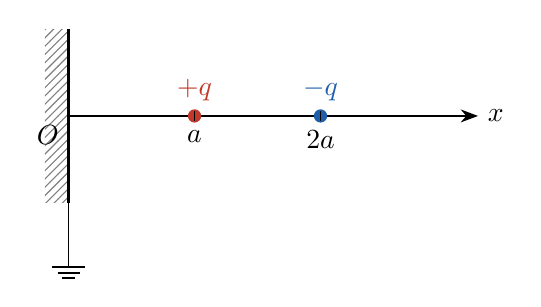
\begin{tikzpicture}[scale=1.0]
  \fill[pattern=north east lines, pattern color=gray] (-0.3,-1.1) rectangle (0,1.1);
  \draw[very thick] (0,-1.1) -- (0,1.1);
  \draw (0,-1.1) -- (0,-1.5) node[ground]{};
  \draw[eje] (0,0) -- (5.2,0) node[right]{$x$};
  \node[below left] at (0,0) {$O$};
  \fill[rojo] (1.6,0) circle (2.4pt) node[above=2pt]{$+q$};
  \fill[azul] (3.2,0) circle (2.4pt) node[above=2pt]{$-q$};
  \draw (1.6,0.06) -- (1.6,-0.06) node[below]{$a$};
  \draw (3.2,0.06) -- (3.2,-0.06) node[below]{$2a$};
\end{tikzpicture}
\end{document}
